\documentclass[8pt,aspectratio=169]{beamer}
\usepackage{minted}

% There are many different themes available for Beamer. A comprehensive
% list with examples is given here:
% http://deic.uab.es/~iblanes/beamer_gallery/index_by_theme.html
% You can uncomment the themes below if you would like to use a different
% one:
%\usetheme{AnnArbor}
%\usetheme{Antibes}
%\usetheme{Bergen}
%\usetheme{Berkeley}
%\usetheme{Berlin}
%\usetheme{Boadilla}
%\usetheme{boxes}
%\usetheme{CambridgeUS}
%\usetheme{Copenhagen}
%\usetheme{Darmstadt}
%\usetheme{default}
%\usetheme{Frankfurt}
%\usetheme{Goettingen}
%\usetheme{Hannover}
%\usetheme{Ilmenau}
%\usetheme{JuanLesPins}
%\usetheme{Luebeck}
\usetheme{Madrid}
%\usetheme{Malmoe}
%\usetheme{Marburg}
%\usetheme{Montpellier}
%\usetheme{PaloAlto}
%\usetheme{Pittsburgh}
%\usetheme{Rochester}
%\usetheme{Singapore}
%\usetheme{Szeged}
%\usetheme{Warsaw}

\title{An Introduction to Functional Programming}

\author{Glenn R. Fisher}
% - Give the names in the same order as the appear in the paper.
% - Use the \inst{?} command only if the authors have different
%   affiliation.

\institute[IBM Mobile Innovation Lab] % (optional, but mostly needed)

% \date{Conference Name, 2013}
% - Either use conference name or its abbreviation.
% - Not really informative to the audience, more for people (including
%   yourself) who are reading the slides online

\subject{Programming Languages}
% This is only inserted into the PDF information catalog. Can be left
% out. 

% If you have a file called "organization-logo-filename.xxx", where xxx
% is a graphic format that can be processed by latex or pdflatex,
% resp., then you can add a logo as follows:

\pgfdeclareimage[height=0.5cm]{organization-logo}{figures/MIL_Logo_BW}
\logo{\pgfuseimage{organization-logo}}

% Delete this, if you do not want the table of contents to pop up at
% the beginning of each subsection:
\AtBeginSubsection[]
{
  \begin{frame}<beamer>{Outline}
    \tableofcontents[currentsection,currentsubsection]
  \end{frame}
}

% Let's get started
\begin{document}

\begin{frame}
  \titlepage
\end{frame}

\begin{frame}{Outline}
  \tableofcontents[pausesections, hideallsubsections]
  % You might wish to add the option [pausesections]
\end{frame}

%%%%%%%%%%%%%%%%%%%%%%%%%%%%%%%%%%%%%%%%%%%%%%%%%%%%%%%%%%%%%%%%%%%%%%%%%%%%%%%%
% Section - What is Functional Programming?
%%%%%%%%%%%%%%%%%%%%%%%%%%%%%%%%%%%%%%%%%%%%%%%%%%%%%%%%%%%%%%%%%%%%%%%%%%%%%%%%

\section{What is Functional Programming?}

%%%%%%%%%%
% Slide
%%%%%%%%%%

\begin{frame}{What is Functional Programming?}

\pause
Functional programming is a different way to think about writing programs.
\newline

\begin{itemize}
\item \pause
  \textbf{First-Class Functions}: A function can return another function or accept functions as parameters.
\item \pause
  \textbf{Lack of State}: There are no assignment statements. Everything is immutable.
\item \pause
  \textbf{Expressions (Not Instructions)}: Functions compute results instead of performing actions.
\item \pause
  \textbf{Comprehensive Type System}: Create types and catch errors at compile time.
\end{itemize}

\vspace{5mm}

\pause
During this talk, we'll try to develop \textbf{intuition} behind these ideas.

\end{frame}

%%%%%%%%%%%%%%%%%%%%%%%%%%%%%%%%%%%%%%%%%%%%%%%%%%%%%%%%%%%%%%%%%%%%%%%%%%%%%%%%
% Section - Why Learn Functional Programming?
%%%%%%%%%%%%%%%%%%%%%%%%%%%%%%%%%%%%%%%%%%%%%%%%%%%%%%%%%%%%%%%%%%%%%%%%%%%%%%%%

\section{Why Learn Functional Programming?}

%%%%%%%%%%
% Slide
%%%%%%%%%%

\begin{frame}{Why Learn Functional Programming?}

\pause
What are the benefits of thinking and programming functionally?
\newline

\begin{itemize}
\item \pause
  Programs are easier to \textbf{understand}.
\item \pause
  Shorter, cleaner, and more \textbf{maintainable} code.
\item \pause
  Fewer errors. Higher \textbf{reliability}.
\item \pause
  Excellent \textbf{performance} with easy parallelism and concurrency.
\end{itemize}

\end{frame}

%%%%%%%%%%%%%%%%%%%%%%%%%%%%%%%%%%%%%%%%%%%%%%%%%%%%%%%%%%%%%%%%%%%%%%%%%%%%%%%%
% Section - Where is Functional Programming Used?
%%%%%%%%%%%%%%%%%%%%%%%%%%%%%%%%%%%%%%%%%%%%%%%%%%%%%%%%%%%%%%%%%%%%%%%%%%%%%%%%

\section{Where is Functional Programming Used?}

%%%%%%%%%%
% Slide
%%%%%%%%%%

\begin{frame}{Where is Functional Programming Used?}

\pause
Companies Using Functional Languages:

\begin{columns}[onlytextwidth]
\begin{column}{0.5\textwidth}
\begin{center}
\begin{itemize}
  \item Twitter
  \item Jane Street Capital
  \item Airbnb
  \item Intel
  \item LinkedIn
\end{itemize}
\end{center}
\end{column}
\begin{column}{0.5\textwidth}
\begin{center}
\begin{itemize}
  \item Foursquare
  \item AT\&T
  \item Bank of America
  \item NVIDIA
  \item And Many More...
\end{itemize}
\end{center}
\end{column}
\end{columns}

\vspace{10mm}

\pause
You don't need to use a functional programming language to think and program functionally.
\newline

\pause
\hspace*{20pt}
Functional Programming != Functional Programming Languages

\pause
\hspace*{20pt}
(Although functional programming languages force you to think functionally.)
\newline

\end{frame}

%%%%%%%%%%%%%%%%%%%%%%%%%%%%%%%%%%%%%%%%%%%%%%%%%%%%%%%%%%%%%%%%%%%%%%%%%%%%%%%%
% Section - Rapid Introduction to Haskell
%%%%%%%%%%%%%%%%%%%%%%%%%%%%%%%%%%%%%%%%%%%%%%%%%%%%%%%%%%%%%%%%%%%%%%%%%%%%%%%%

\section{Rapid Introduction to Haskell}

%%%%%%%%%%%%%%%%%%%%%%%%%%%%%%%%%%%%%%%%%%%%%%%%%%%%%%%%%%%%%%%%%%%%%%%%%%%%%%%%
% Section - Rapid Introduction to Haskell
% Subsection - Variables
%%%%%%%%%%%%%%%%%%%%%%%%%%%%%%%%%%%%%%%%%%%%%%%%%%%%%%%%%%%%%%%%%%%%%%%%%%%%%%%%

\subsection{Variables}

%%%%%%%%%%
% Slide
%%%%%%%%%%

\begin{frame}[fragile]{Rapid Introduction to Haskell: Variables}

\pause
\begin{minted}{haskell}
x :: Integer
x = 3
\end{minted}

\pause
\begin{minted}{haskell}
pi :: Double
pi = 3.1415926
\end{minted}

\pause
\begin{minted}{haskell}
b1, b2 :: Bool
b1 = True
b2 = False
\end{minted}

\end{frame}

%%%%%%%%%%%%%%%%%%%%%%%%%%%%%%%%%%%%%%%%%%%%%%%%%%%%%%%%%%%%%%%%%%%%%%%%%%%%%%%%
% Section - Rapid Introduction to Haskell
% Subsection - Arithmetic
%%%%%%%%%%%%%%%%%%%%%%%%%%%%%%%%%%%%%%%%%%%%%%%%%%%%%%%%%%%%%%%%%%%%%%%%%%%%%%%%

\subsection{Arithmetic}

%%%%%%%%%%
% Slide
%%%%%%%%%%

\begin{frame}[fragile]{Rapid Introduction to Haskell: Arithmetic}

\pause
\begin{minted}{haskell}
ex01 = 3 + 2
\end{minted}

\pause
\begin{minted}{haskell}
ex02 = 19 - 27
\end{minted}

\pause
\begin{minted}{haskell}
ex03 = 2.35 * 8.6
\end{minted}

\pause
\begin{minted}{haskell}
ex04 = 8.7 / 3.1
\end{minted}

\pause
\begin{minted}{haskell}
ex05 = div 12 5
\end{minted}

\pause
\begin{minted}{haskell}
ex06 = 7 ^ 222
\end{minted}

\end{frame}

%%%%%%%%%%%%%%%%%%%%%%%%%%%%%%%%%%%%%%%%%%%%%%%%%%%%%%%%%%%%%%%%%%%%%%%%%%%%%%%%
% Section - Rapid Introduction to Haskell
% Subsection - A Note on Parentheses
%%%%%%%%%%%%%%%%%%%%%%%%%%%%%%%%%%%%%%%%%%%%%%%%%%%%%%%%%%%%%%%%%%%%%%%%%%%%%%%%

\subsection{A Note on Parentheses}

%%%%%%%%%%
% Slide
%%%%%%%%%%

\begin{frame}[fragile]{Rapid Introduction to Haskell: A Note on Parentheses}

\pause
Many languages use parentheses to call functions.

\pause
\begin{minted}{java}
    sum(3, 4, 5);
\end{minted}

\vspace{5mm}

\pause
In Haskell, we omit the parentheses and use spaces instead.

\pause
\begin{minted}{haskell}
    sum 3 4 5
\end{minted}

\vspace{5mm}

\pause
However, we may need parentheses to compute an argument before calling the function.

\pause
\begin{minted}{haskell}
    sum (1 + 2) 4 5
\end{minted}

\end{frame}

%%%%%%%%%%%%%%%%%%%%%%%%%%%%%%%%%%%%%%%%%%%%%%%%%%%%%%%%%%%%%%%%%%%%%%%%%%%%%%%%
% Section - Rapid Introduction to Haskell
% Subsection - Boolean Logic
%%%%%%%%%%%%%%%%%%%%%%%%%%%%%%%%%%%%%%%%%%%%%%%%%%%%%%%%%%%%%%%%%%%%%%%%%%%%%%%%

\subsection{Boolean Logic}

%%%%%%%%%%
% Slide
%%%%%%%%%%

\begin{frame}[fragile]{Rapid Introduction to Haskell: Boolean Logic}

\pause
\begin{minted}{haskell}
ex07 = True && False
\end{minted}

\pause
\begin{minted}{haskell}
ex08 = not (True || False)
\end{minted}

\pause
\begin{minted}{haskell}
ex09 = ('a' == 'a')
\end{minted}

\pause
\begin{minted}{haskell}
ex10 = (16 /= 3)
\end{minted}

\pause
\begin{minted}{haskell}
ex11 = "Haskell" > "C++"
\end{minted}

\end{frame}

%%%%%%%%%%%%%%%%%%%%%%%%%%%%%%%%%%%%%%%%%%%%%%%%%%%%%%%%%%%%%%%%%%%%%%%%%%%%%%%%
% Section - Rapid Introduction to Haskell
% Subsection - Functions
%%%%%%%%%%%%%%%%%%%%%%%%%%%%%%%%%%%%%%%%%%%%%%%%%%%%%%%%%%%%%%%%%%%%%%%%%%%%%%%%

\subsection{Functions}

%%%%%%%%%%
% Slide
%%%%%%%%%%

\begin{frame}[fragile]{Rapid Introduction to Haskell: Functions}

\pause
\begin{minted}{haskell}
doubleMe :: Integer -> Integer
doubleMe x = x + x
\end{minted}

\pause
\begin{minted}{haskell}
quadrupleMe :: Integer -> Integer
quadrupleMe x = doubleMe (doubleMe x)
\end{minted}

\end{frame}

%%%%%%%%%%
% Slide
%%%%%%%%%%

\begin{frame}[fragile]{Rapid Introduction to Haskell: Functions}

We can also write functions with local variables.

\pause
\begin{minted}{haskell}
hypotenuse :: Double -> Double -> Double
hypotenuse length width = sqrt squaredHypotenuse
  where squaredHypotenuse = length^2 + width^2
\end{minted}

\pause
\begin{minted}{haskell}
hypotenuse2 :: Double -> Double -> Double
hypotenuse2 length width =
  let squaredHypotenuse = length^2 + width^2 in
  sqrt squaredHypotenuse
\end{minted}

\end{frame}

%%%%%%%%%%%%%%%%%%%%%%%%%%%%%%%%%%%%%%%%%%%%%%%%%%%%%%%%%%%%%%%%%%%%%%%%%%%%%%%%
% Section - Rapid Introduction to Haskell
% Subsection - Types
%%%%%%%%%%%%%%%%%%%%%%%%%%%%%%%%%%%%%%%%%%%%%%%%%%%%%%%%%%%%%%%%%%%%%%%%%%%%%%%%

\subsection{Types}

%%%%%%%%%%
% Slide
%%%%%%%%%%

\begin{frame}[fragile]{Rapid Introduction to Haskell: Types}

\pause
\begin{minted}{haskell}
type Position = (Double, Double)
\end{minted}

\pause
\begin{minted}{haskell}
position :: Position
position = (1.25, 2.75)
\end{minted}

\pause
\begin{minted}{haskell}
magnitude :: Position -> Double
magnitude (x, y) = sqrt (x * x + y * y)
\end{minted}

\vspace{5mm}

\pause
(We will return to this example later.)

\end{frame}

%%%%%%%%%%
% Slide
%%%%%%%%%%

\begin{frame}[fragile]{Rapid Introduction to Haskell: Types}

\pause
A Person has a name, age, and favorite color.

\pause
\begin{minted}{haskell}
type Name = String
\end{minted}

\pause
\begin{minted}{haskell}
type Age = Integer
\end{minted}

\pause
\begin{minted}{haskell}
type Color = String
\end{minted}

\pause
\begin{minted}{haskell}
data Person = Person Name Age Color
\end{minted}

\pause
\begin{minted}{haskell}
glenn :: Person
glenn = Person "Glenn R. Fisher" 22 "Green"
\end{minted}

\pause
\begin{minted}{haskell}
favoriteColor :: Person -> Color
favoriteColor (Person name age color) = color
\end{minted}

\pause
\begin{minted}{haskell}
favoriteColor glenn == "Green"
\end{minted}

\end{frame}

%%%%%%%%%%%%%%%%%%%%%%%%%%%%%%%%%%%%%%%%%%%%%%%%%%%%%%%%%%%%%%%%%%%%%%%%%%%%%%%%
% Section - Example: Position
%%%%%%%%%%%%%%%%%%%%%%%%%%%%%%%%%%%%%%%%%%%%%%%%%%%%%%%%%%%%%%%%%%%%%%%%%%%%%%%%

\section{Example: Position}

%%%%%%%%%%
% Slide
%%%%%%%%%%

\begin{frame}[fragile]{Position}

Let's create a Position type and write associated functions.
\newline

\pause
\begin{minted}{haskell}
{- a Distance is a length in space -}
type Distance = Double
\end{minted}

\pause
\begin{minted}{haskell}
{- a Position is a pair of x and y distances -}
type Position = (Distance, Distance)
\end{minted}

\pause
\begin{minted}{haskell}
{- reflect returns a new Position reflected over the origin -}
reflect :: Position -> Position
reflect (x, y) = (-x, -y)
\end{minted}

\pause
\begin{minted}{haskell}
{- magnitude returns a Position's distance from the origin -}
magnitude :: Position -> Distance
magnitude (x, y) = sqrt (x * x + y * y)
\end{minted}

\pause
\begin{minted}{haskell}
{- translate returns a new Position translated by an offset -}
translate :: Position -> Position -> Position
translate (x, y) (offsetX, offsetY) = (x + offsetX, y + offsetY)
\end{minted}

\end{frame}

%%%%%%%%%%%%%%%%%%%%%%%%%%%%%%%%%%%%%%%%%%%%%%%%%%%%%%%%%%%%%%%%%%%%%%%%%%%%%%%%
% Section - Example: Region
%%%%%%%%%%%%%%%%%%%%%%%%%%%%%%%%%%%%%%%%%%%%%%%%%%%%%%%%%%%%%%%%%%%%%%%%%%%%%%%%

\section{Example: Region}

%%%%%%%%%%
% Slide
%%%%%%%%%%

\begin{frame}[fragile]{Example: Region}

Let's create a Region type and write associated functions.

\pause
How should we represent a region in 2D space?

\begin{columns}[onlytextwidth]
\begin{column}{0.45\textwidth}

\pause
\begin{center}
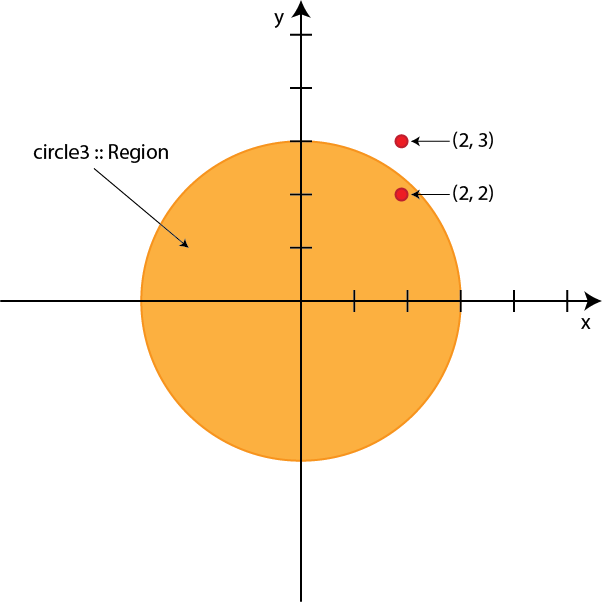
\includegraphics[scale=0.3]{figures/region}
\end{center}

\end{column}
\begin{column}{0.55\textwidth}

\pause
\begin{minted}{haskell}
type Region = Position -> Bool
\end{minted}

\pause
\begin{minted}{haskell}
circle3 (2, 2) == True
\end{minted}

\pause
\begin{minted}{haskell}
circle3 (2, 3) == False
\end{minted}

\pause
\begin{minted}{haskell}
circle3 :: Region
circle3 position = (magnitude position <= 3.0)
\end{minted}

\pause
\begin{minted}{haskell}
circle4 :: Region
circle4 position = (magnitude position <= 4.0)
\end{minted}

\pause
\begin{minted}{haskell}
circle :: Distance -> Region
circle radius = fun
  where fun position = (magnitude position <= radius)
\end{minted}

\pause
\begin{minted}{haskell}
easyCircle3 = circle 3.0
easyCircle4 = circle 4.0
\end{minted}

\end{column}
\end{columns}

\end{frame}

%%%%%%%%%%
% Slide
%%%%%%%%%%

\begin{frame}[fragile]{Example: Region}

What if we don't want our circle to be centered at the origin?

\begin{columns}[onlytextwidth]
\begin{column}{0.5\textwidth}
\pause
\begin{center}
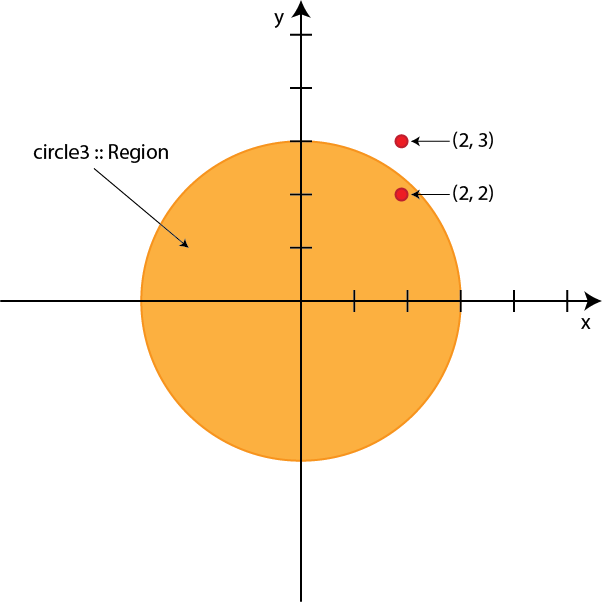
\includegraphics[scale=0.22]{figures/region}
\end{center}
\end{column}
\begin{column}{0.5\textwidth}
\pause
\begin{center}
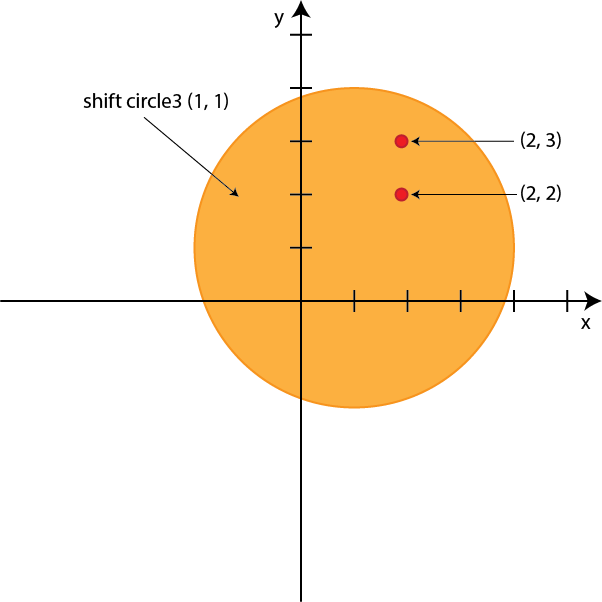
\includegraphics[scale=0.22]{figures/shiftedRegion}
\end{center}
\end{column}
\end{columns}

\vspace{3mm}

% avoid spacing between subsequent lines in block
\setlength\partopsep{-\topsep}
\addtolength\partopsep{-\parskip}
\addtolength\partopsep{0.1cm}

\pause
\begin{minted}{haskell}
{- shift transforms a region by translating it by an offset -}
shift :: Region -> Position -> Region
\end{minted}

\pause
\begin{minted}{haskell}
shift region offset = fun
  where fun position = region (translate position (reflect offset))
\end{minted}

% reset spacing between subsequent lines in block
\setlength\partopsep{2pt}

\end{frame}

%%%%%%%%%%
% Slide
%%%%%%%%%%

\begin{frame}[fragile]{Example: Region}

What if we want the region outside of the circle?

\begin{columns}[onlytextwidth]
\begin{column}{0.5\textwidth}
\pause
\begin{center}
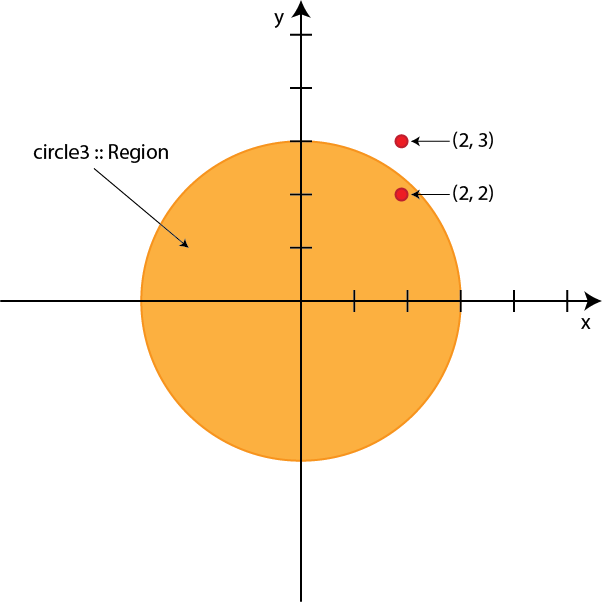
\includegraphics[scale=0.22]{figures/region}
\end{center}
\end{column}
\begin{column}{0.5\textwidth}
\pause
\begin{center}
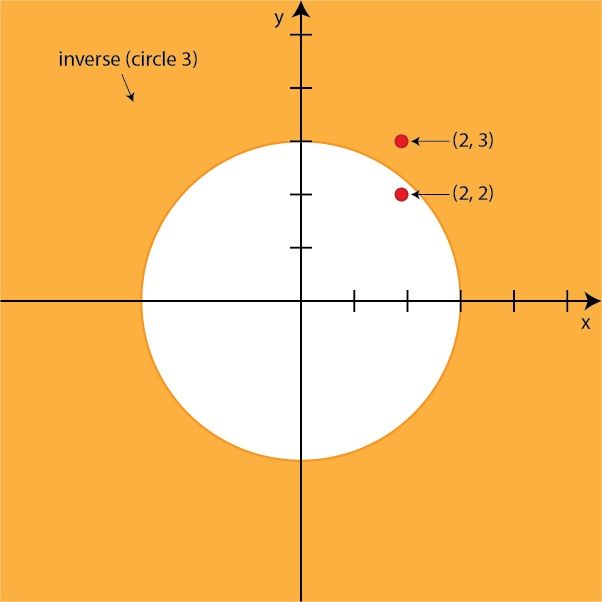
\includegraphics[scale=0.22]{figures/invertedRegion}
\end{center}
\end{column}
\end{columns}

\vspace{3mm}

% avoid spacing between subsequent lines in block
\setlength\partopsep{-\topsep}
\addtolength\partopsep{-\parskip}
\addtolength\partopsep{0.1cm}

\pause
\begin{minted}{haskell}
{- invert transforms a region by inverting the set of Positions that it contains -}
invert :: Region -> Region
\end{minted}

\pause
\begin{minted}{haskell}
invert region = fun
    where fun position = not (region position)
\end{minted}

% reset spacing between subsequent lines in block
\setlength\partopsep{2pt}

\end{frame}

%%%%%%%%%%
% Slide
%%%%%%%%%%

\begin{frame}[fragile]{Example: Region}

Can we combine regions to create new regions?

\begin{columns}[onlytextwidth]
\begin{column}{0.5\textwidth}
\pause
\begin{center}
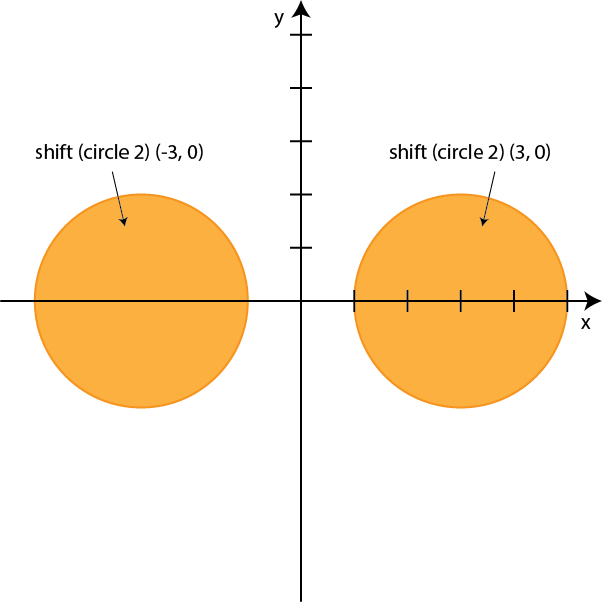
\includegraphics[scale=0.22]{figures/unionRegion1}
\end{center}
\end{column}
\begin{column}{0.5\textwidth}
\pause
\begin{center}
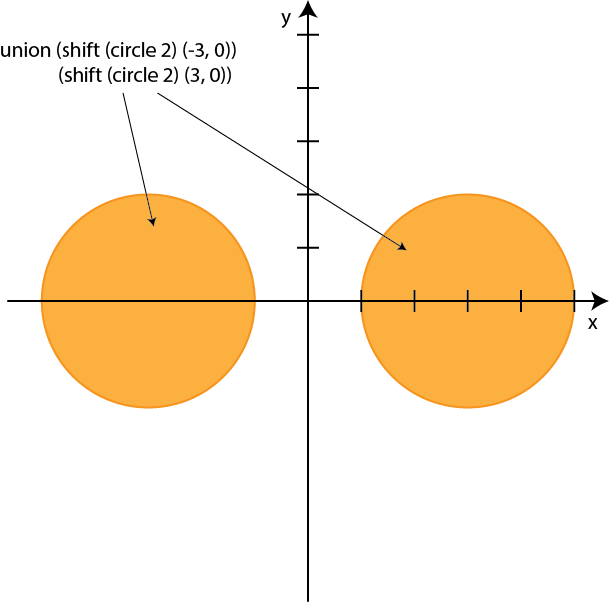
\includegraphics[scale=0.22]{figures/unionRegion2}
\end{center}
\end{column}
\end{columns}

\vspace{3mm}

% avoid spacing between subsequent lines in block
\setlength\partopsep{-\topsep}
\addtolength\partopsep{-\parskip}
\addtolength\partopsep{0.1cm}

\pause
\begin{minted}{haskell}
{- union constructs a new Region from the union of two Regions -}
union :: Region -> Region -> Region
\end{minted}

\pause
\begin{minted}{haskell}
union region1 region2 = fun
    where fun position = (region1 position) || (region2 position)
\end{minted}

% reset spacing between subsequent lines in block
\setlength\partopsep{2pt}

\end{frame}

%%%%%%%%%%
% Slide
%%%%%%%%%%

\begin{frame}[fragile]{Example: Region}

Can we combine regions to create new regions?

\begin{columns}[onlytextwidth]
\begin{column}{0.5\textwidth}
\pause
\begin{center}
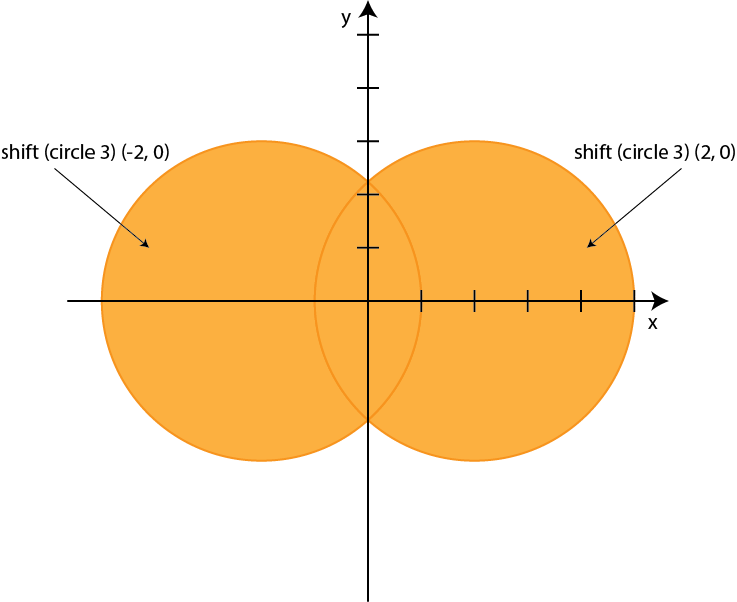
\includegraphics[scale=0.22]{figures/intersectionRegion1}
\end{center}
\end{column}
\begin{column}{0.5\textwidth}
\pause
\begin{center}
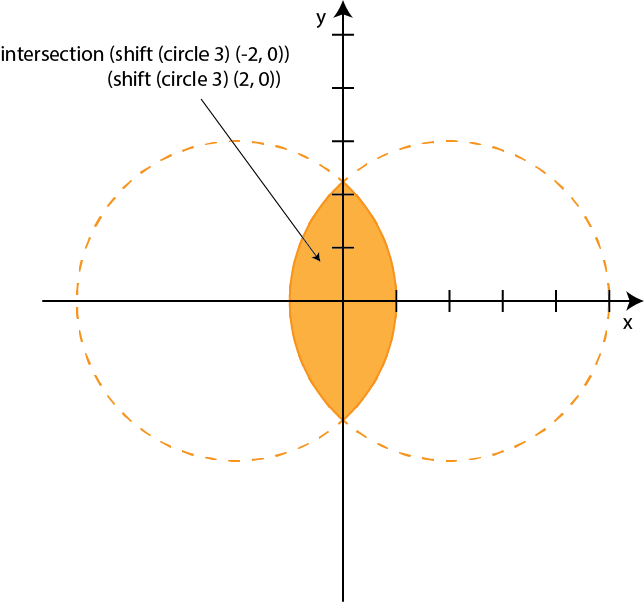
\includegraphics[scale=0.22]{figures/intersectionRegion2}
\end{center}
\end{column}
\end{columns}

\vspace{3mm}

% avoid spacing between subsequent lines in block
\setlength\partopsep{-\topsep}
\addtolength\partopsep{-\parskip}
\addtolength\partopsep{0.1cm}

\pause
\begin{minted}{haskell}
{- intersection constructs a new Region from the intersection of two Regions -}
intersection :: Region -> Region -> Region
\end{minted}

\pause
\begin{minted}{haskell}
intersection region1 region2 = fun
    where fun position = (region1 position) && (region2 position)
\end{minted}

% reset spacing between subsequent lines in block
\setlength\partopsep{2pt}

\end{frame}

%%%%%%%%%%
% Slide
%%%%%%%%%%

\begin{frame}[fragile]{Example: Region}

Can we combine regions to create new regions?

\begin{columns}[onlytextwidth]
\begin{column}{0.5\textwidth}
\pause
\begin{center}
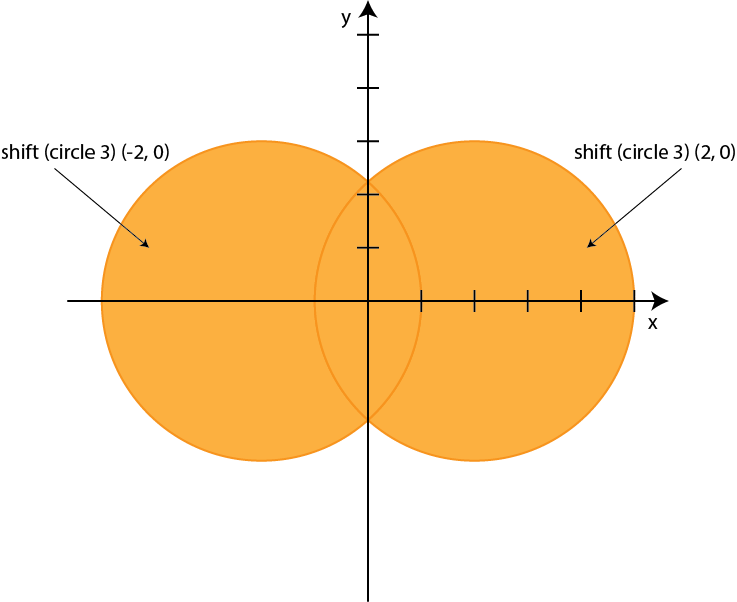
\includegraphics[scale=0.22]{figures/diffRegion1}
\end{center}
\end{column}
\begin{column}{0.5\textwidth}
\pause
\begin{center}
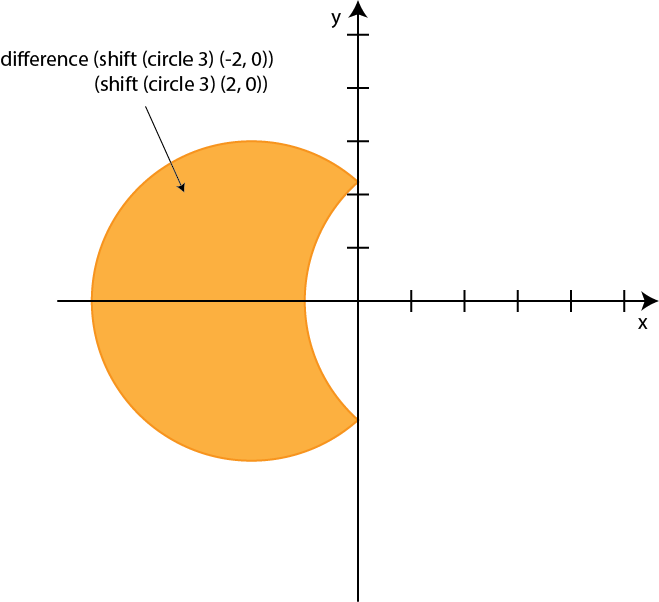
\includegraphics[scale=0.22]{figures/diffRegion2}
\end{center}
\end{column}
\end{columns}

\vspace{3mm}

% avoid spacing between subsequent lines in block
\setlength\partopsep{-\topsep}
\addtolength\partopsep{-\parskip}
\addtolength\partopsep{0.1cm}

\pause
\begin{minted}{haskell}
{- difference constructs a new Region containing all the Positions
   of the first region that are not members of the second Region -}
difference :: Region -> Region -> Region
\end{minted}

\pause
\begin{minted}{haskell}
difference region minus = 
    intersection region (invert minus)
\end{minted}

% reset spacing between subsequent lines in block
\setlength\partopsep{2pt}

\end{frame}

%%%%%%%%%%
% Slide
%%%%%%%%%%

\begin{frame}[fragile]{Example: Region}

Let's create a Region type and write associated functions.
\newline

\pause
\begin{minted}{haskell}
{- A Region is a set of Positions and is defined by a function that
   determines whether a given Position is a member of the set -}
type Region = Position -> Bool
\end{minted}

\pause
\begin{minted}{haskell}
{- circle returns a circular Region with the given radius, centered at the origin -}
circle :: Distance -> Region
circle radius = fun
    where fun position = (magnitude position <= radius)
\end{minted}

\pause
\begin{minted}{haskell}
{- shift transforms a region by translating it by an offset -}
shift :: Region -> Position -> Region
shift region offset = fun
    where fun position = region (translate position (reflect offset))
\end{minted}

\pause
\begin{minted}{haskell}
{- invert transforms a region by inverting the set of Positions that it contains -}
invert :: Region -> Region
invert region = fun
    where fun position = not (region position)
\end{minted}

\end{frame}

%%%%%%%%%%
% Slide
%%%%%%%%%%

\begin{frame}[fragile]{Example: Region}

\begin{minted}{haskell}
{- intersection constructs a new Region from the intersection of two Regions -}
intersection :: Region -> Region -> Region
intersection region1 region2 = fun
    where fun position = (region1 position) && (region2 position)
\end{minted}

\pause
\begin{minted}{haskell}
{- union constructs a new Region from the union of two Regions -}
union :: Region -> Region -> Region
union region1 region2 = fun
    where fun position = (region1 position) || (region2 position)
\end{minted}

\pause
\begin{minted}{haskell}
{- difference constructs a new Region containing all the Positions
   of the first region that are not members of the second Region -}
difference :: Region -> Region -> Region
difference region minus = 
    intersection region (invert minus)
\end{minted}

\end{frame}

%%%%%%%%%%%%%%%%%%%%%%%%%%%%%%%%%%%%%%%%%%%%%%%%%%%%%%%%%%%%%%%%%%%%%%%%%%%%%%%%
% Section - Summary
%%%%%%%%%%%%%%%%%%%%%%%%%%%%%%%%%%%%%%%%%%%%%%%%%%%%%%%%%%%%%%%%%%%%%%%%%%%%%%%%

\section{Summary}

%%%%%%%%%%
% Slide
%%%%%%%%%%

\begin{frame}{Summary}

Functional programming is a different way to think about writing programs.
\newline

\begin{itemize}
\item
  \textbf{First-Class Functions}: A function can return another function or accept functions as parameters.
\item
  \textbf{Lack of State}: There are no assignment statements. Everything is immutable.
\item
  \textbf{Expressions (Not Instructions)}: Functions compute results instead of performing actions.
\item
  \textbf{Comprehensive Type System}: Create types and catch errors at compile time.
\end{itemize}

\vspace{5mm}

Hopefully this talk helped you develop \textbf{intuition} behind these ideas.

\end{frame}

\end{document}

%%%%%%%%%%%%%%%%%%%%%%%%%%%%%%%%%%%%%%%%%%%%%%%%%%%%%%%%%%%%%%%%%%%%%%%%%%%%%%%%
% Tips and tricks from template
%%%%%%%%%%%%%%%%%%%%%%%%%%%%%%%%%%%%%%%%%%%%%%%%%%%%%%%%%%%%%%%%%%%%%%%%%%%%%%%%

% % You can reveal the parts of a slide one at a time
% % with the \pause command:
% \begin{frame}{Second Slide Title}
%   \begin{itemize}
%   \item {
%     First item.
%     \pause % The slide will pause after showing the first item
%   }
%   \item {   
%     Second item.
%   }
%   % You can also specify when the content should appear
%   % by using <n->:
%   \item<3-> {
%     Third item.
%   }
%   \item<4-> {
%     Fourth item.
%   }
%   % or you can use the \uncover command to reveal general
%   % content (not just \items):
%   \item<5-> {
%     Fifth item. \uncover<6->{Extra text in the fifth item.}
%   }
%   \end{itemize}
% \end{frame}

% \begin{frame}{Blocks}
% \begin{block}{Block Title}
% You can also highlight sections of your presentation in a block, with it's own title
% \end{block}
% \begin{theorem}
% There are separate environments for theorems, examples, definitions and proofs.
% \end{theorem}
% \begin{example}
% Here is an example of an example block.
% \end{example}
% \end{frame}

% % Placing a * after \section means it will not show in the
% % outline or table of contents.
% \section*{Summary}

% \begin{frame}{Summary}
%   \begin{itemize}
%   \item
%     The \alert{first main message} of your talk in one or two lines.
%   \item
%     The \alert{second main message} of your talk in one or two lines.
%   \item
%     Perhaps a \alert{third message}, but not more than that.
%   \end{itemize}
  
%   \begin{itemize}
%   \item
%     Outlook
%     \begin{itemize}
%     \item
%       Something you haven't solved.
%     \item
%       Something else you haven't solved.
%     \end{itemize}
%   \end{itemize}
% \end{frame}

% % All of the following is optional and typically not needed. 
% \appendix
% \section<presentation>*{\appendixname}
% \subsection<presentation>*{For Further Reading}

% \begin{frame}[allowframebreaks]
%   \frametitle<presentation>{For Further Reading}
    
%   \begin{thebibliography}{10}
    
%   \beamertemplatebookbibitems
%   % Start with overview books.

%   \bibitem{Author1990}
%     A.~Author.
%     \newblock {\em Handbook of Everything}.
%     \newblock Some Press, 1990.
 
    
%   \beamertemplatearticlebibitems
%   % Followed by interesting articles. Keep the list short. 

%   \bibitem{Someone2000}
%     S.~Someone.
%     \newblock On this and that.
%     \newblock {\em Journal of This and That}, 2(1):50--100,
%     2000.
%   \end{thebibliography}
% \end{frame}
